%%%%%%%%%%%%%%%%%%%%%%%%%%%%%%%%%%%%%%%%%
% Stylish Article
% LaTeX Template
% Version 2.1 (1/10/15)
%
% This template has been downloaded from:
% http://www.LaTeXTemplates.com
%
% Original author:
% Mathias Legrand (legrand.mathias@gmail.com) 
% With extensive modifications by:
% Vel (vel@latextemplates.com)
%
% License:
% CC BY-NC-SA 3.0 (http://creativecommons.org/licenses/by-nc-sa/3.0/)
%
%%%%%%%%%%%%%%%%%%%%%%%%%%%%%%%%%%%%%%%%%

%----------------------------------------------------------------------------------------
%	PACKAGES AND OTHER DOCUMENT CONFIGURATIONS
%----------------------------------------------------------------------------------------

\documentclass[fleqn,10pt]{SelfArx} % Document font size and equations flushed left

\usepackage[english]{babel} % Specify a different language here - english by default

\usepackage{lipsum} % Required to insert dummy text. To be removed otherwise
\usepackage[bookmarks=true,pdfborder={0 0 0}]{hyperref}
\hypersetup{colorlinks=TRUE,linkbordercolor=red,linkcolor=green,pdfborderstyle={/S/U/W 1}}
\usepackage{amsmath} 
\usepackage{textcomp}
\usepackage{url}



%----------------------------------------------------------------------------------------
%	COLUMNS
%----------------------------------------------------------------------------------------

\setlength{\columnsep}{0.55cm} % Distance between the two columns of text
\setlength{\fboxrule}{0.75pt} % Width of the border around the abstract

%----------------------------------------------------------------------------------------
%	COLORS
%----------------------------------------------------------------------------------------

\definecolor{color1}{RGB}{0,0,90} % Color of the article title and sections
\definecolor{color2}{RGB}{0,20,20} % Color of the boxes behind the abstract and headings

%----------------------------------------------------------------------------------------
%	HYPERLINKS
%----------------------------------------------------------------------------------------

\usepackage{hyperref} % Required for hyperlinks
\hypersetup{hidelinks,colorlinks,breaklinks=true,urlcolor=color2,citecolor=color1,linkcolor=color1,bookmarksopen=false,pdftitle={Title},pdfauthor={Author}}

%----------------------------------------------------------------------------------------
%	ARTICLE INFORMATION
%----------------------------------------------------------------------------------------

\JournalInfo{Computational and Linguistic Analysis L545 Spring 2017} % Journal information
\Archive{} % Additional notes (e.g. copyright, DOI, review/research article)

\PaperTitle{Using Named Entity Recognition technique to classify News Articles} % Article title

\Authors{Ankit Saxena, Shailendra Patil} % Authors

\Keywords{Classification --- Support Vector Machines ---  Part of Speech Tagging  --- Chunking --- Named Entity Recognition  } % Keywords - if you don't want any simply remove all the text between the curly brackets
\newcommand{\keywordname}{Keywords} % Defines the keywords heading name

%----------------------------------------------------------------------------------------
%	ABSTRACT
%----------------------------------------------------------------------------------------

\Abstract{This project deals with classifying the news articles. In this project we take the "The Reuters-21578, Distribution 1.0" data. There are total 135 classes into which the news has been classified. The training data has already been classified, our task is to classify the articles from test data into its corresponding classes. We have applied three different methods to train the data. First we implemented the model by training it using Support Vector Machine (SVM), but before applying the SVM we normalized and tokenized the data in all articles and then trained the model using SVM. In the second approach, we used Named entity recognition. In this part we first did the Part of Speech (POS) tagging of words and based on POS tags we did the Named Entity Extraction. In the third approach, we have used the Noun Phrase chunks to normalize the text. Using the tokenized data from the text we have trained our model using SVM. Finally we compare the results of the three methods described above.}

%----------------------------------------------------------------------------------------

\begin{document}

\flushbottom % Makes all text pages the same height

\maketitle % Print the title and abstract box

\tableofcontents % Print the contents section

\thispagestyle{empty} % Removes page numbering from the first page

%----------------------------------------------------------------------------------------
%	ARTICLE CONTENTS
%----------------------------------------------------------------------------------------

\section*{Introduction} % The \section*{} command stops section numbering
As the number of news articles and texts are increasing significantly on a daily basis, it is becoming a great challenge for newspapers to categorize or determine the interest of their users. Given the fact that most of the news these days is consumed electronically, we need an algorithm to classify the news automatically. In this project, we have classified the news article using Named Entity Recognition, Noun Phrase chunking and a traditional data normalization technique. Named-entity recognition (NER, also known as entity identification, entity chunking and entity extraction) is a subtask of information extraction that seeks to locate and classify named entities in text into predefined categories such as the names of persons, organizations, locations, expressions of times, quantities, monetary values, percentages, etc \cite{REF:1}. \textbf{The Reuters-21578, Distribution 1.0} data is used for our analysis.  Using the various techniques for text normalization and tokenization, we have generated multi-label classification models and used them to predict the labels of the articles in the test dataset.
\addcontentsline{toc}{section}{Introduction} % Adds this section to the table of contents

%------------------------------------------------

\section{Theory}
\subsection{Tokenization}
 Tokenization is the process of breaking a stream of text up into words, phrases, symbols, or other meaningful elements called tokens. The list of tokens becomes input for further processing such as parsing or text mining \cite{REF:2}.
\\\textbf{Example} : "Lets make America great again. The White House is in United States. My friend lives in a white house. A White House is beautiful."
 \\We will use the same example for future references.
\\This is how Tokenization applied on the above sentence looks like :
\begin{figure}[h]
\begin{minipage}[b]{1.0\linewidth}
  \centering
  \centerline{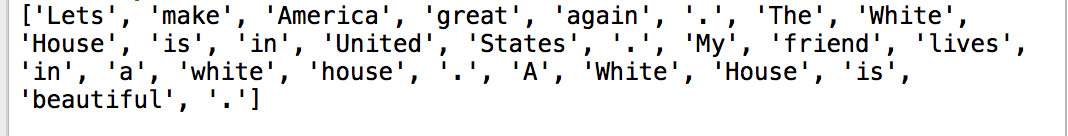
\includegraphics[width=9cm]{token}}
%  \vspace{2.0cm}
  \centerline{Figure 1. Tokenization}\medskip
\end{minipage}
\end{figure}

\newpage

Typically, tokenization occurs at the word level. The tokenized words can be used for further analysis, like one can do POS tagging on the tokenized words, and can also perform chunking, named entity recognition etc.
\\We have used the \textbf{word\_tokenize} from \textbf{NLTK} for Tokenization

\subsection{POS Tagging}
In corpus linguistics, \textbf{part-of-speech tagging} (POS tagging or POST), also called grammatical tagging or word-category disambiguation, is the process of marking up a word in a text (corpus) as corresponding to a particular part of speech, based on both its definition and its context$-$i.e., its relationship with adjacent and related words in a phrase, sentence, or paragraph \cite{REF:3}.
\\\\For the same example considered above, once Tokenization is done, we applied POS tagging on the tokenized words. Below is the results obtained for the same: 
\begin{figure}[h]
\begin{minipage}[b]{1.0\linewidth}
  \centering
  \centerline{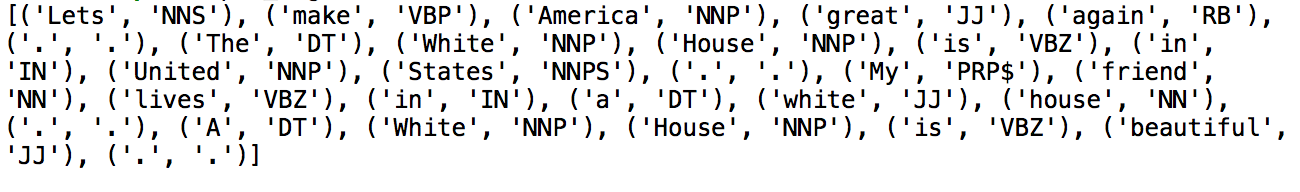
\includegraphics[width=9cm]{postags}}
%  \vspace{2.0cm}
  \centerline{Figure 2. POS  Tags}\medskip
\end{minipage}
\end{figure}
\\ \textbf{pos\_tag} from {nltk} was used for this process. POS tagged words can be further used to obtain chunks, a process known as \textbf{Chunking}.

\subsection{Chunking}
Chunking is also called shallow parsing and it's basically the identification of parts of speech and short phrases (like noun phrases). Part of speech tagging tells you whether words are nouns, verbs, adjectives, etc, but it doesn't give you any clue about the structure of the sentence or phrases in the sentence. Using chunking technique, we can get the Noun Phrase Chunks(NP), Verb Phrase Chunks(VP) etc. Chunking find its application in Named Entity Recognition \cite{REF:4}.
\begin{figure}[h]
\begin{minipage}[b]{1.0\linewidth}
  \centering
  \centerline{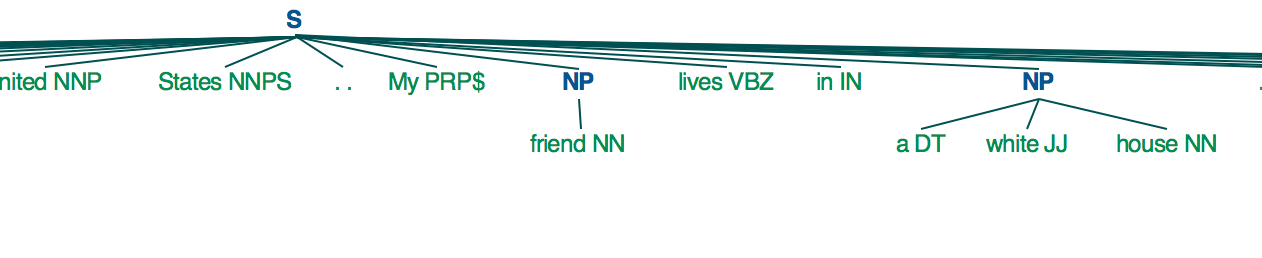
\includegraphics[width=9cm]{chunks}}
%  \vspace{2.0cm}
  \centerline{Figure 3. NP Chunks}\medskip
\end{minipage}
\end{figure}
\\In the example mentioned earlier, a white house is one among the NP phrases. We have used regular expression on POS tagged data to get the NP phrases.

\subsection{Named Entity Recognition}
Named-entity recognition (NER, also known as entity identification, entity chunking and entity extraction) is a subtask of information extraction that seeks to locate and classify named entities in text into pre-defined categories such as the names of persons, organizations, locations, expressions of times, quantities, monetary values, percentages, etc \cite{REF:1}.
\textbf{ne\_chunks} from \textbf{NLTK} was used for this purpose. The various named entity tags are shown below \cite{REF:9}: 
\begin{figure}[h]
\begin{minipage}[b]{1.0\linewidth}
  \centering
  \centerline{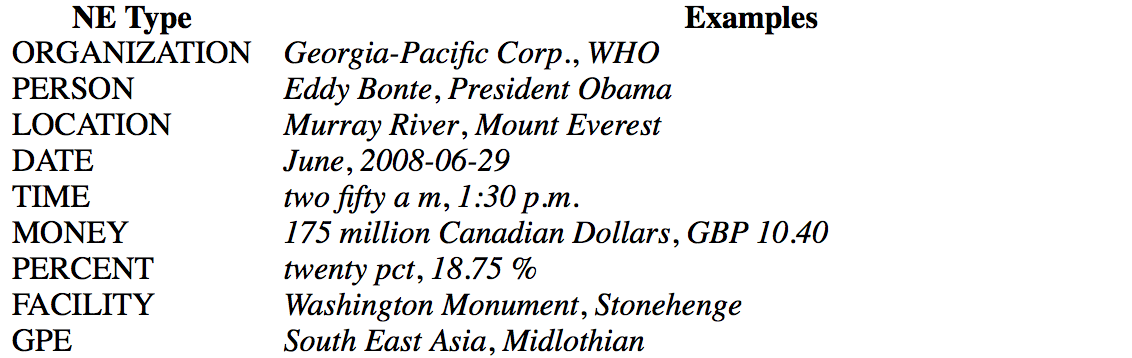
\includegraphics[width=9cm]{nertags}}
%  \vspace{2.0cm}
  \centerline{Figure 4. NER Tags}\medskip
\end{minipage}
\end{figure}
\\\\For the example considered, below are few Named entity recognized in the text.
\begin{figure}[h]
\begin{minipage}[b]{1.0\linewidth}
  \centering
  \centerline{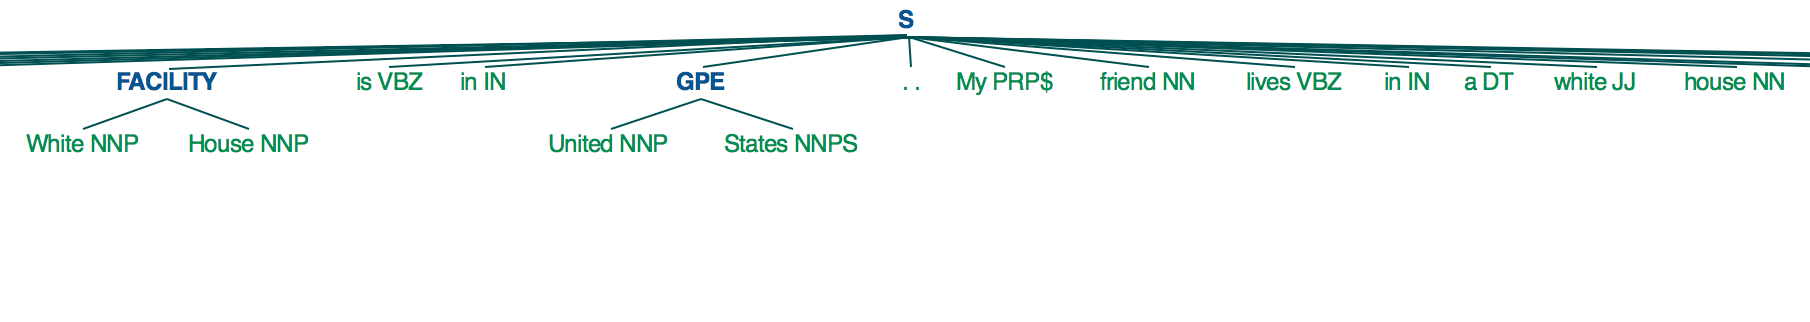
\includegraphics[width=9cm]{nertree}}
%  \vspace{2.0cm}
  \centerline{Figure 5. NER Tree}\medskip
\end{minipage}
\end{figure}
\\\\Here \textbf{White House} is tagged as \textbf{FACILITY}. But in the sentence we have "a white house", here it is not treated as \textbf{FACILITY}. It can be seen that the Named Entity recognition depends on the context as well.
\subsection{Support Vector Machines}
In our project we are using \textbf{Support Vector Machine(SVM)} for training and making predictions. In machine learning, SVM's are supervised learning models with associated learning algorithms that analyze data used for classification and regression analysis. Given a set of training examples, each marked as belonging to one or the other of two categories, an SVM training algorithm builds a model that assigns new examples to one category or the other, making it a non-probabilistic binary linear classifier \cite{REF:6}. 
\\\\In other words, given labeled training data (supervised learning), the algorithm outputs an optimal hyperplane which categorizes new examples.
\\\\Below is typical example for two classes classification and the number of splits it can have. It can be seen that there are many possible hyperplanes that correctly classifies the data. The goal of SVM is to find the optimal hyperplane among all the possible hyperplanes.

\begin{center}
\begin{figure}
\begin{minipage}[b]{1.0\linewidth}
  \centering
  \centerline{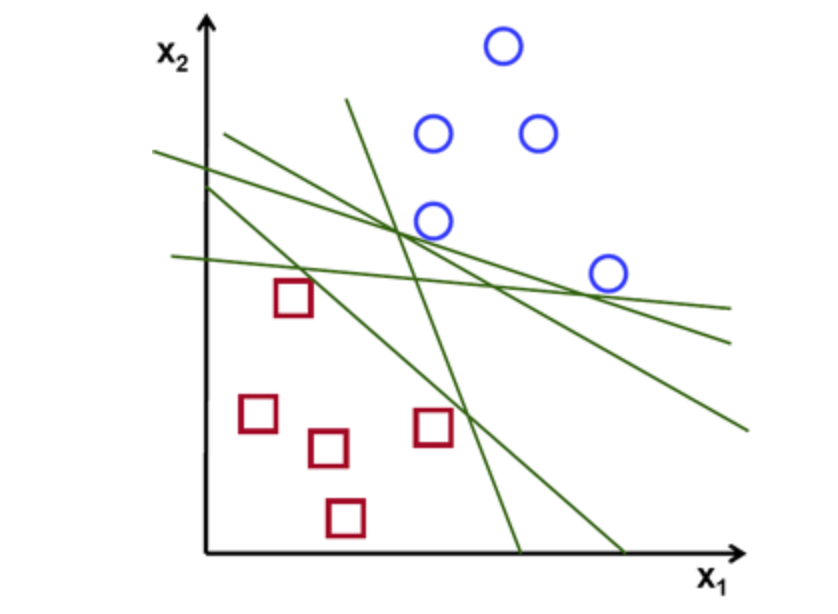
\includegraphics[width=9cm]{SVM}}
%  \vspace{2.0cm}
  \centerline{Figure 6. Classification}\medskip
\end{minipage}
\end{figure}
\end{center}

\newpage

\section{Data}

%\begin{equation}
%\cos^3 \theta =\frac{1}{4}\cos\theta+\frac{3}{4}\cos 3\theta
%\label{eq:refname2}
%\end{equation}

\subsection{Data Background}
\textbf{The Reuters-21578, Distribution 1.0} \cite{REF:5} dataset is used for our analysis. The documents in the Reuters-21578 collection appeared on the Reuters newswire in 1987. The documents were assembled and indexed with categories by personnel from \textbf{Reuters Ltd.} (Sam Dobbins, Mike Topliss, Steve Weinstein) and Carnegie Group, Inc. (Peggy Andersen, Monica Cellio, Phil Hayes, Laura Knecht, Irene Nirenburg) in 1987.
\\\\In 1990, the documents were made available by \textbf{Reuters} and \textbf{CGI} for research purposes to the Information Retrieval Laboratory (W.  Bruce Croft, Director) of the Computer and Information Science Department at the University of Massachusetts at Amherst.  Formatting of the documents and production of associated data files was done in 1990 by \textbf{David D.  Lewis} and \textbf{Stephen Harding} at the Information Retrieval Laboratory.
\\\\Further formatting and data file production was done in 1991 and 1992 by David D. Lewis and Peter Shoemaker at the Center for Information and Language Studies, University of Chicago.  This version of the data was made available for anonymous FTP as "Reuters-22173, Distribution 1.0" in January 1993. From 1993 through 1996, Distribution 1.0 was hosted at a succession of FTP sites maintained by the Center for Intelligent Information Retrieval (W. Bruce Croft, Director) of the Computer Science Department at the University of Massachusetts at Amherst.


\subsection{Data Description}
The dataset consists of \textbf{22 data files}, along with \textbf{SGML Document Type Definition} file that describes the data file
format, and \textbf{six} other files describing the categories used to index the data. The documents have a \textbf{unique ID}
number which is assigned in chronological order to the data files starting from 1, with each data file consisting of
\textbf{1000} documents ordered by this unique ID.\\\\The data files are in \textbf{SGML} format. Each file begins with a document type declaration line. All individual articles
are marked with SGML tags, $<$REUTERS$>$ is the starting tag and $</$REUTERS$>$ is the ending tag.
The \textbf{document id} can be identified by the \textbf{NEWID} value within the REUTERS tag. This value is unique for every news article.
\\\\For every \textbf{document id}, we have one or more topic(s) defined for it, which is/are present within the $<$TOPICS$>$ tag. There are a total of \textbf{135} unique topics into which the documents are classified.
\\\\These 135 topics are saved in \textbf{"all$-$topics$-$strings.lc.txt"} file. Every document used in our training model is labeled with one or more of these 135 values. 
\\\\The content of the document is found within the $<$BODY$>$ tag. Every document id has a BODY, which contains the article content. In our analysis,  Topics, Doc id and Body are tags that are of prime importance.
\subsection{Data Preprocessing}
The biggest task in any Text Mining problem is Data Preprocessing. Before we apply any algorithms, we first need to clean the data.  The 22 files has the data in SGML format. So we first need to extract the data without any tags. So first we clean the data such that for every document id, we only take the body of the document along with topic associated  with it and save it as \textbf{csv (comma separated value)} file. The body of the document is converted as bag of words and then saved into the csv file.  Figure1 is the representation of how the csv file looks and how it is saved.
\begin{figure}[h]
\begin{minipage}[b]{1.0\linewidth}
  \centering
  \centerline{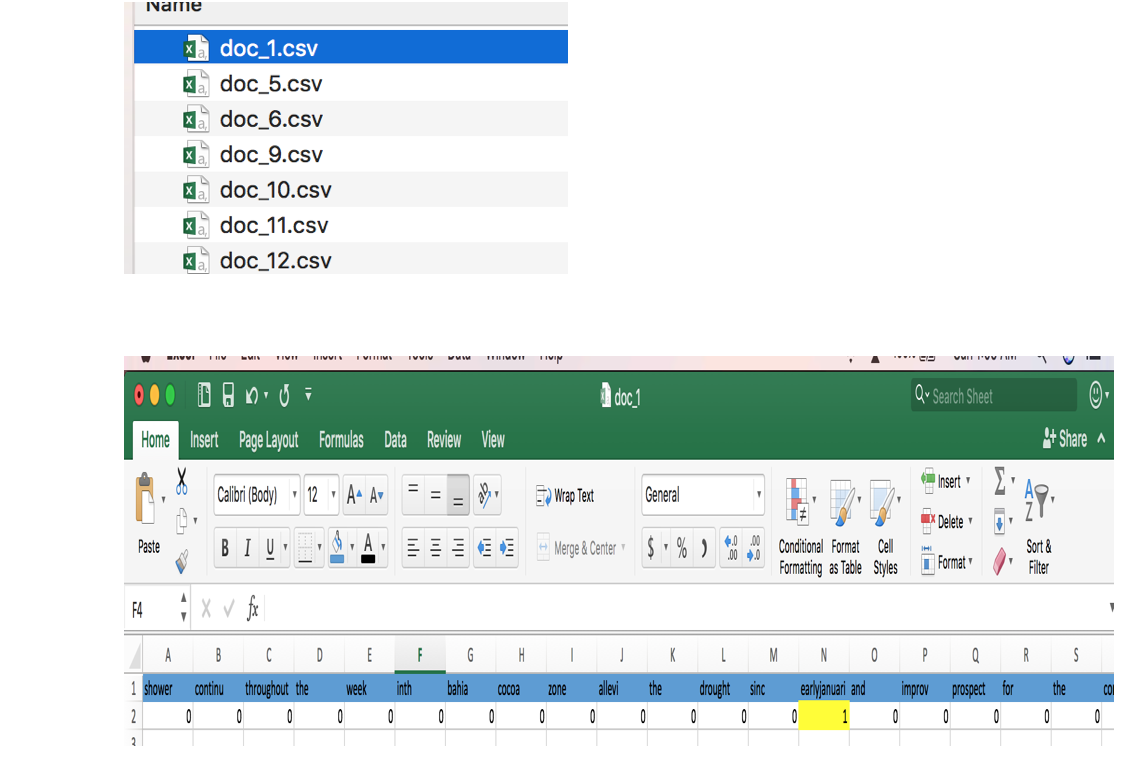
\includegraphics[width=8cm]{representation}}
%  \vspace{2.0cm}
  \centerline{Figure 7. Representation of data after removing tags}\medskip
\end{minipage}
\end{figure}
\\As seen, \textbf{doc$\_1$.csv} represents the csv file created from document id 1, the file name general syntax is \textbf{doc$\_$documentid.csv}. The content of the csv file is as shown. The \textbf{blue} highlighted row is the bag of words from that particular document, row \textbf{1} in this case. And the second row is a list of \textbf{135} values representing the topics. These 135 values list are in the same order in which topics are saved in \textbf{"all$-$topics$-$strings.lc.txt"} . The second row values will be either \textbf{0} or \textbf{1}. If the value of a column is 1, then the corresponding column number should be checked with column number as row number of \textbf{"all$-$topics$-$strings.lc.txt"} and that particular topic or topics would be the \textbf{classification} of the given document. In the figure, \textbf{yellow} entry represents 1 and it is in \textbf{14th column}. When we check the textbf{"all$-$topics$-$strings.lc.txt"} 14th row, we find it is \textbf{cocoa}. So the \textbf{document id 1} classification is \textbf{cocoa}.

%------------------------------------------------
\phantomsection
\section{Experiment}
In this section we discuss the flow of the experiment along with the implementation process. Figure 6 shows a typical \textbf{flow chart}. Here we implement our project in two different methods as show in the flow chart:
\begin{enumerate}
\item \textbf{Method1}: Here we used a traditional approach of preprocessing, like tokenizing the words and removing stop words and applying the learning algorithm.
\item \textbf{Method2}: We use NP Chunks and Named Entity Recognition for data preprocessing and then apply the learning algorithm.
\end{enumerate}
\begin{figure}
\begin{minipage}[b]{1.0\linewidth}
  \centering
  \centerline{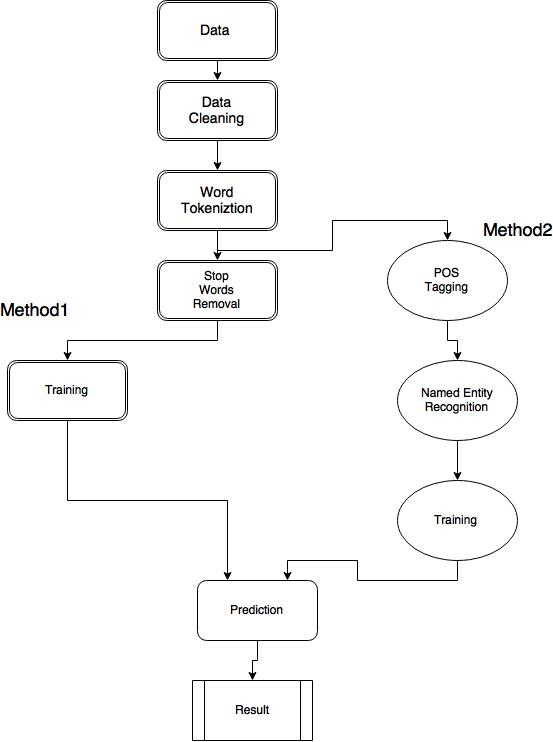
\includegraphics[width=8cm]{Flowchart2}}
%  \vspace{2.0cm}
  \centerline{Figure 8. Flow Chart}\medskip
\end{minipage}
\end{figure}
The flow chart can be explained as:
\begin{enumerate}
\item
\textbf{Data}: In this problem, we have a total of 135 labels for the newspaper articles. Each article can be labeled with more than one label.
\\\\In order to classify the documents, we need to learn or build a model from the documents that are already labeled. We need to extract meaningful information or words here, from these documents and use their actual labels as a means for the accuracy check.
\item \textbf{Data Preprocessing}:
Below explanation we consider data cleaning, word tokenization, POS tagging, named entity recognition as a part of Data Preprocessing. We have a dataset with multiple labels under the category 'topics'. We have used One-vs-Rest technique with SVM (Polynomial and RBF kernel) for text classification. First, a vocabulary was made for the words that occur in the documents that are already labeled and this vocabulary has been used as a feature vector for the model.
\\\\The dictionary has been made in three different ways, first with simple preprocessing, second with Named Entity extraction, and the third one with Noun Phrase chunking.
\\\\For the three approaches, we have used \textbf{OneVsRestClassifier} from the \textbf{sklearn.multiclass} library to classify the documents into multiple labels. The predicted output is a vector of size 135 labels for each document, where label(i) = 1 denotes that the document belong to that $i^{th}$ label of topics.
\\\\The data in the dataset is present inside XML tags with SGML file format. The documents are either categorized with a label under 'topics' or not. We have used only the documents that are categorized under at least one 'topic'. Each SGML file has been parsed and the useful data has been extracted using the XML tags. The 'body' tag data was extracted and data cleaning steps were applied on it. The data cleaning techniques differ for the three methods used for vocabulary building. The vocabulary is generated for the 135 labels under the 'topics' category by taking the union of the vocab list. Each document has been stored in the 'files' directory for further processing.
\\File to be executed: $1\textunderscore create\textunderscore mapping\textunderscore*.ipynb$.
\\\\After generating the individual vocabulary files for each label, we create a consolidated vocabulary or the union of all the vocabs. This works as our feature vector. A vector of size equal to the words in the consolidated vocabulary is created and we enter "1" for the word index which occur in the body tag, for each document. The consolidated vocabulary is stored in the file, $"vocab\_main.csv"$ \cite{REF:8}.
\\File to be executed: $2\textunderscore create\textunderscore vocab.ipynb$.
\\\\Using the saved labeled documents we have created a feature matrix with each document as a row in the matrix and the column are the feature vectors corresponding to the consolidated vocabulary. The feature matrix along with expected output is stored in the matrices form on the local drive, as $"X\_train.mat"$ for the feature matrix and $Y\textunderscore train.mat$ for the expected output. The size of the $"X\_train.mat"$ is number of documents * size of consolidated vocabulary. The size of the $"Y\_train.mat"$ is number of documents * number of labels. File to be executed: $3\textunderscore train\textunderscore data.ipynb$.
\\\\We have made the consolidated dictionary in three different ways, first with simple preprocessing (traditional approach), second with Named Entity extraction, and the third with Noun Phrase chunking.
\begin{enumerate}
\item \textbf{Simple preprocessing}
The following techniques have been used to normalize the text in the \textbf{body} tag in the given sequence:
Convert the text to lowercase, remove all the HTML tags, remove the numbers, process URL, process email address, process dollar sign, remove punctuations. After these steps, we have Tokenized the text by splitting with $'\ '$. The non-alphanumeric characters are removed and all the word stem are extracted for each word, using the \textbf{PorterStemmer} from \textbf{nltk.stem} package. The stop have not been removed from this list of stem words.
\item\textbf{Named Entity extraction}
The following techniques have been used to normalize the text in the \textbf{body} tag in the given sequence:
Remove all the HTML tags, remove the numbers, process URL, process email address, process dollar sign, remove non-alphanumeric characters. After these steps, we have found the Named Entities, using the \textbf{ne\_chunk} from nltk package. After this, we have converted all the extracted Named Entities to lowercase.
\item\textbf{Noun Phrase chunking}
The following techniques have been used to normalize the text in the \textbf{body} tag in the given sequence:
Remove all the HTML tags, remove the numbers, process URL, process email address, process dollar sign, remove non-alphanumeric characters. After these steps, we have found the NP chunks, using the \textbf{pos\_tag} from nltk package and regular expression. After this, we have converted all the extracted NP chunks to lowercase.
\end{enumerate}
Using the saved matrices, we have split the data into train and test with the help of $train\textunderscore test\textunderscore split$ library from \\$sklearn.cross\_validation$. We have 70 $\%$ of the data for training purpose and 30$\%$ for testing. \textbf{OneVsRestClassifier} from the \textbf{sklearn.multiclass} library is used to train the model. First, we have used Polynomial kernel to train the model and then used RBF kernel. The value for accuracy, precision and recall are calculated. 
\\File to be executed: $4\textunderscore SVM\textunderscore classify.ipynb$.
\\\\To create a classifier for a new dataset or unlabeled data, we need to follow the above steps and train the model on the entire training data above instead of just 70$\%$. The test data would be the unlabeled data.
\item \textbf{Training and Prediction}
Using the saved matrices, we have split the data into train and test with the help of $train\textunderscore test\textunderscore split$ library from \\$sklearn.cross\_validation$. We have 70 $\%$ of the data for training purpose and 30$\%$ for testing. \textbf{OneVsRestClassifier} from the \textbf{sklearn.multiclass} library is used to train the model. First, we have used Polynomial kernel to train the model and then used RBF kernel. The value for accuracy, precision and recall are calculated. 
\\File to be executed: $4\textunderscore SVM\textunderscore classify.ipynb$.
\\\\To create a classifier for a new dataset or unlabeled data, we need to follow the above steps and train the model on the entire training data above instead of just 70$\%$. The test data would be the unlabeled data. Using the model trained on test data , we predict the classed of unlabeled data.
\end{enumerate}

\section{Observations}
For the three different consolidated dictionaries, we have observed the Precision and Recall for the two models, and calculated the time taken to train the model and predict the labels. Out of the 135 labels, we have provided the Precision-Recall curve for the first label as an example and the Precision-Recall curve for all the labels combined (for RBF model).
\begin{enumerate}
\item \textbf{Simple preprocessing}
\\Vocabulary Size: 3711 words
\\\\SVM (Polynomial)
\\ \begin{tabular}{|c c c c|} 
\hline
Accuracy & Precision & Recall & Time Taken(s)\\ \hline
99.0651 & 1.0 & 0.000292 & 780.1743 \\ \hline
\end{tabular}
\\\\\\SVM (RBF)
\\Time Taken(sec): 2751.6169

\begin{figure}

\begin{minipage}[b]{1.0\linewidth}
  \centering
  \centerline{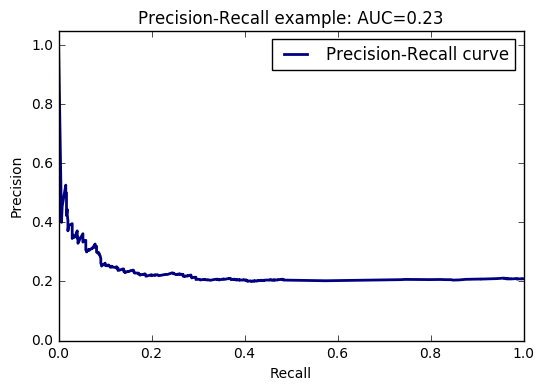
\includegraphics[width=9cm]{SampleGraphLabel1}}
%  \vspace{2.0cm}
  \centerline{Figure 9. PR curve for Simple preprocessing (Label 1)}\medskip
\end{minipage}

\begin{minipage}[b]{1.0\linewidth}
  \centering
  \centerline{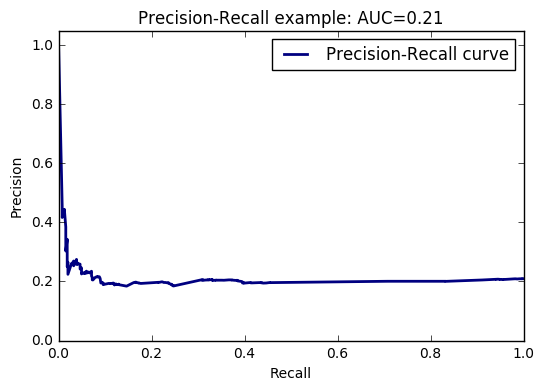
\includegraphics[width=9cm]{SampleGraphLabel2}}
%  \vspace{2.0cm}
  \centerline{Figure 11. PR curve for Named Entity extraction (Label 1)}\medskip
\end{minipage}

\begin{minipage}[b]{1.0\linewidth}
  \centering
  \centerline{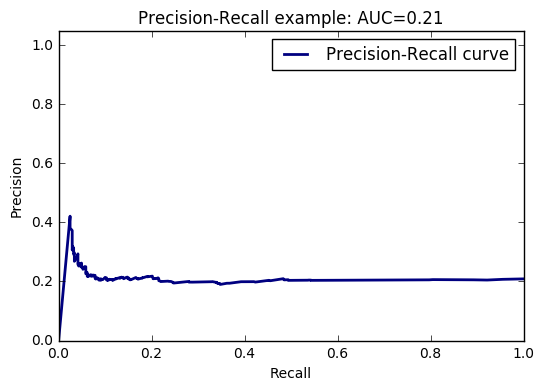
\includegraphics[width=9cm]{SampleGraphLabel3}}
%  \vspace{2.0cm}
  \centerline{Figure 13. PR curve for Noun Phrase chunking (Label 1)}\medskip
\end{minipage}

\end{figure}


\begin{figure}

\begin{minipage}[b]{1.0\linewidth}
  \centering
  \centerline{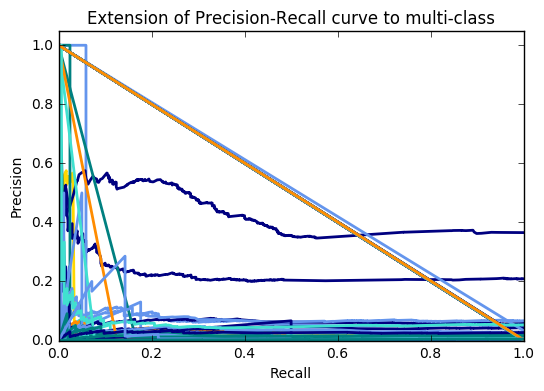
\includegraphics[width=9cm]{MulticlassPvsR1}}
%  \vspace{2.0cm}
  \centerline{Figure 10. PR curve for Simple preprocessing (all labels)}\medskip
\end{minipage}

\begin{minipage}[b]{1.0\linewidth}
  \centering
  \centerline{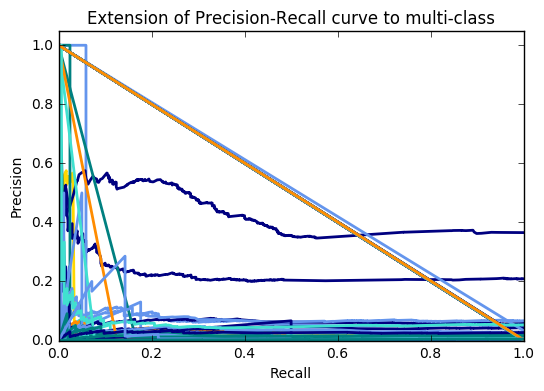
\includegraphics[width=9cm]{MulticlassPvsR1}}
%  \vspace{2.0cm}
  \centerline{Figure 12. PR curve for Named Entity extraction (all labels)}\medskip
\end{minipage}

\begin{minipage}[b]{1.0\linewidth}
  \centering
  \centerline{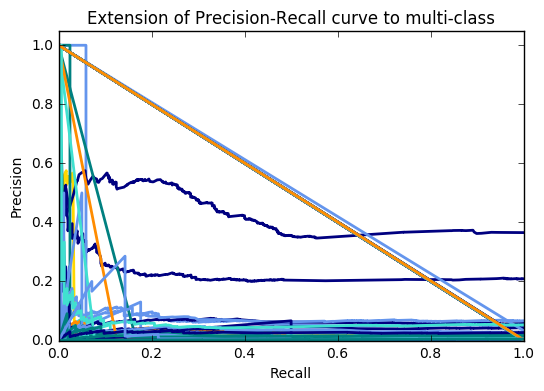
\includegraphics[width=9cm]{MulticlassPvsR1}}
%  \vspace{2.0cm}
  \centerline{Figure 14. PR curve for Noun Phrase chunking (all labels)}\medskip
\end{minipage}

\end{figure}


\item\textbf{Named Entity extraction}
\\Vocabulary Size: 590 words
\\\\SVM (Polynomial)
\\ \begin{tabular}{|c c c c|} 
\hline
Accuracy & Precision & Recall & Time Taken(s)\\ \hline
99.0651 & 1.0 & 0.000292 & 122.5908 \\ \hline
\end{tabular}
\\\\\\SVM (RBF)
\\Time Taken(sec): 480.3060


\item\textbf{Noun Phrase chunking}
\\Vocabulary Size: 1094 words
\\\\SVM (Polynomial)
\\ \begin{tabular}{|c c c c|} 
\hline
Accuracy & Precision & Recall & Time Taken(s)\\ \hline
99.0646 & 1.0 & 0.000288 & 232.6776 \\ \hline
\end{tabular}
\\\\\\SVM (RBF)
\\Time Taken(sec): 885.3276
\end{enumerate}

\textbf{Interpretation}: Recall is a performance measure of the entire positive part of a dataset whereas Precision is a performance measure of the positive predictions. The value of AUC (area under the curve) lies between 0 and 1 and a higher value denotes a better prediction model.
\\\\In our experiment, we found the value of AUC to be very small. All the three dictionaries have presented similar results, but the prediction with Named Entity recognition takes less time and consumes less storage compared to the other two \cite{REF:7}.

\section{Future Work}
We would like to improve the efficiency of the data cleaning process by refining the text normalization process, fine tune the model parameters, to improve the precision and recall of the models.
\\\\We would also like to implement other Machine Learning techniques like Bayes Classifier, Artificial Neural Networks to train the model and compare the results with our observations.

%------------------------------------------------
\phantomsection
\section*{Acknowledgments} % The \section*{} command stops section numbering

\addcontentsline{toc}{section}{Acknowledgments} % Adds this section to the table of contents
We have put in considerable efforts to reach this stage of the project but it would not have been possible without the continuous guidance and support of many other individuals. We would like to extend our sincere thanks to all of them.
\\ \\ We are highly indebted to our Professor \href{http://cl.indiana.edu/~md7/}{Markus Dickinson}, for his supervision as well as for providing the necessary resources required for the completion of this project report.

\newpage

%----------------------------------------------------------------------------------------
%	REFERENCE LIST
%----------------------------------------------------------------------------------------
\phantomsection

\bibliographystyle{unsrt}
\bibliography{report}

%----------------------------------------------------------------------------------------

\end{document}